\documentclass{article}


% Paquetes
\usepackage[utf8]{inputenc}
\usepackage[T1]{fontenc}
\usepackage[spanish]{babel}
\usepackage[left=2.5cm,right=2.5cm,top=2.5cm,bottom=2.5cm]{geometry}
\usepackage{titlesec}
\usepackage{lipsum}
\usepackage{graphicx}
\usepackage[ruled,linesnumbered]{algorithm2e}

% Configuración de títulos
\titleformat{\section}{\normalfont\Large\bfseries}{\thesection}{1em}{}
\titleformat{\subsection}{\normalfont\large\bfseries}{\thesubsection}{1em}{}
\titleformat{\subsubsection}{\normalfont\normalsize\bfseries}{\thesubsubsection}{1em}{}


% Título
\title{Informe sobre la solución planteada sobre el "Problema del Agente Viajero"}
\author{Luis Antonio Mamani Alave}
\date{\today}

\begin{document}

\maketitle

\section{Introducción}
El problema del agente viajero es un desafio clásico en el área de la optimización combinatoria y a su vez con diversas aplicaciones practicas. El problema consiste en encontrar la ruta más  optima que permita a un visitante visitar un conjunto de ubicaciones y regresar al punto de partida. Aunque parece sencillo su complejidad rádica en todas las posibles combinaciones de rutas. que aumenta de manera exponencial con el número de ubicaciones planteadas. \\
Para dar solución a este problema se han planteado distintos tipos de algoritmos como los algoritmos exactos que buscan encontrar una solución óptima, evaluando todas las posibles combinaciones. Sin embargo, a medida que aumenta el número de ubicaciones, la complejidad computacional se vuelve desproporcionada. Por otro lado, tambien tenemos los enfoques heuristicos y metaheuristicos, a través de algoritmos genéticos, busqueda de cuervos entre otros, que ofrecen soluciones aprosimadas en tiempos auqnue no garantizan la solución óptima pero si aceptable. 

\section{Objetivos}
El objetivo del trabajo fue, plantear un algoritmo que brinde una solución al problema del agente viajero, utilizando enfoques heurísticos que nos permiten obtener una solución aceptable. Para este caso utilizamos un algoritmo genético.
\newpage
\section{Algoritmo}

\begin{algorithm}[h]
  \caption{Ejemplo de algoritmo}
  \KwData{ciudades, poblacion,generaciones}
  Generamos las rutas aleatorias\;
  \For{$i \leftarrow 1$ \KwTo $generaciones$}{
    Ordenamos las rutas en base a su distancia\;
    Generamos la elite,padres, descendencia\;
    \While{descendencia < poblacion - elite}{
      Seleccionamos aleatoriamente dos padres\;
      Generamos un hijo\;
      \If{probabilidad de mutación}{
          Mutamos al hijo\;
      }
      Agregamos al hijo a la descendencia\;
    }
    poblacion = padres + descendencia\;
  }
  Seleccionamos la mejor ruta\;
  \KwResult{Devolvemos la mejor ruta}
  \caption{Mi algoritmo}
  \end{algorithm}
\section{Implementacion}

\section{Resultados}
Para poder probar el algoritmo planteado utlizamos 3 grupos de ciudades. El primero formado por 5 ciudades, el segundo formado por 10 ciudades y finalmente el tercero formado por 20 ciudades.

\begin{table}[ht]
  \centering
  \caption{Primer Grupo}
  \begin{tabular}{|c|c|c|c|c|c|}
    \hline
    \textbf{Ciudad} & A & B & C & D& E \\
    \hline
    \textbf{Coordenadas} & 0,0 & 1,2 & 3,1 & 5,2 & 3,4\\
    \hline
  \end{tabular}
\end{table}

\begin{table}[ht]
  \centering
  \caption{Segundo Grupo}
  \begin{tabular}{|c|c|c|c|c|c|c|c|c|c|c|}
    \hline
    \textbf{Ciudad} & A & B & C & D & E & F & G & H & I & J \\
    \hline
    \textbf{Coordenadas} & 0,0 & 1,2 & 3,1 & 5,2 & 3,4 & 8,7 & 6,5 & 1,8 & 3,10 & 7,9\\
    \hline
  \end{tabular}
\end{table}

\begin{table}[ht]
  \centering
  \caption{Tercer Grupo}
  \begin{tabular}{|c|c|c|c|c|c|c|c|c|c|c|}
    \hline
    \textbf{Ciudad} & A & B & C & D & E & F & G & H & I & J \\
    \hline
    \textbf{Coordenadas} & 0,0 & 1,2 & 3,1 & 5,2 & 3,4 & 8,7 & 6,5 & 1,8 & 3,10 & 7,9\\
    \hline
  \end{tabular}
  \begin{tabular}{|c|c|c|c|c|c|c|c|c|c|c|}
    \hline
    \textbf{Ciudad} & K & L & M & N & O & P & Q & R & S & T \\
    \hline
    \textbf{Coordenadas} & 0, 1 & 5, 6 & 3, 9 & 5, 10 & 3, 11 & 8, 2 & 6, 1 & 1, 5 & 2, 6 & 4,7\\
    \hline
  \end{tabular}
\end{table}

\newpage
\subsection{Resultados del primer grupo}

Para el primer grupo se realizaron 10 iteraciones sobre un conjunto de 5 ubicaciones, dando como resultados los datos obtenidos en el Cuadro 4.

  \begin{table}[h]
    \centering
    \caption{Resultados de procesamiento del Primer Grupo}
    \begin{tabular}{|c|c|c|c|c|}
      \hline
      \textbf{Nro} & \textbf{P. Inicio} & \textbf{Orden de Visita} & \textbf{Distancia} & \textbf{Tiempo (s)}\\
      \hline
      1 & B: [1, 2] & B, E, D, C, A & 13.2913 & 0.8596 \\
      \hline
      2 & E: [3, 4] & E, B, A, C, D & 13.2913 & 0.8812 \\
      \hline
      3 & D: [5, 2] & D, E, B, A, C & 13.2913 & 0.8755 \\
      \hline
      4 & A: [0, 0] & A, B, E, D, C & 13.2913 & 0.8788 \\
      \hline
      5 & D: [5, 2] & D, C, A, B, E & 13.2913 & 0.9102 \\
      \hline
      6 & A: [0, 0] & A, C, D, E, B & 13.2913 & 0.9030 \\
      \hline
      7 & D: [5, 2] & D, C, A, B, E & 13.2913 & 0.9091 \\
      \hline
      8 & E: [3, 4] & E, D, C, A, B & 13.2913 & 0.9461 \\
      \hline
      9 & E: [3, 4] & E, D, C, A, B & 13.2913 & 0.8779 \\
      \hline
      10 & E: [3, 4] & E, B, A, C, D & 13.2913 & 1.1982 \\
      \hline
    \end{tabular}
  \end{table}

  Como podemos observar en el Cuadro 4, al ser el número de ubicaciones a visitar solo 5 todas las iteraciones muestrane la misma distancia aceptable, a pesar de que el recorrido se realice de distinta manera, en cuanto al tiempo de procesamiento este tiene una media de 0.9240 segundos, mientras que la distancia optima en general es de 13.2913. Así como se muestra en la Figura 1 donde podemos ver la evolucion de la mejor distancia en la quinta iteracion, en donde la distancia no varia.\\

    \begin{figure}[h]
    \centering
    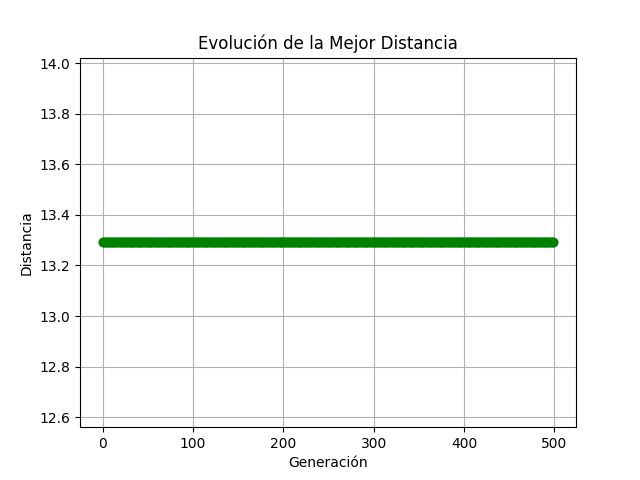
\includegraphics[width=9cm]{img/5Generacion.png}
    \caption{Evolución de la mejor distancia en la quinta iteración.}
    \label{fig:etiqueta1}
  \end{figure}

  En cuanto a la ruta óptima como apreciamos en la Figura 2, esta no muestra ninguna variacion con la de las demás iteraciones a pesar de iniciar de un punto distinto en cada caso.

  \begin{figure}[h]
    \centering
    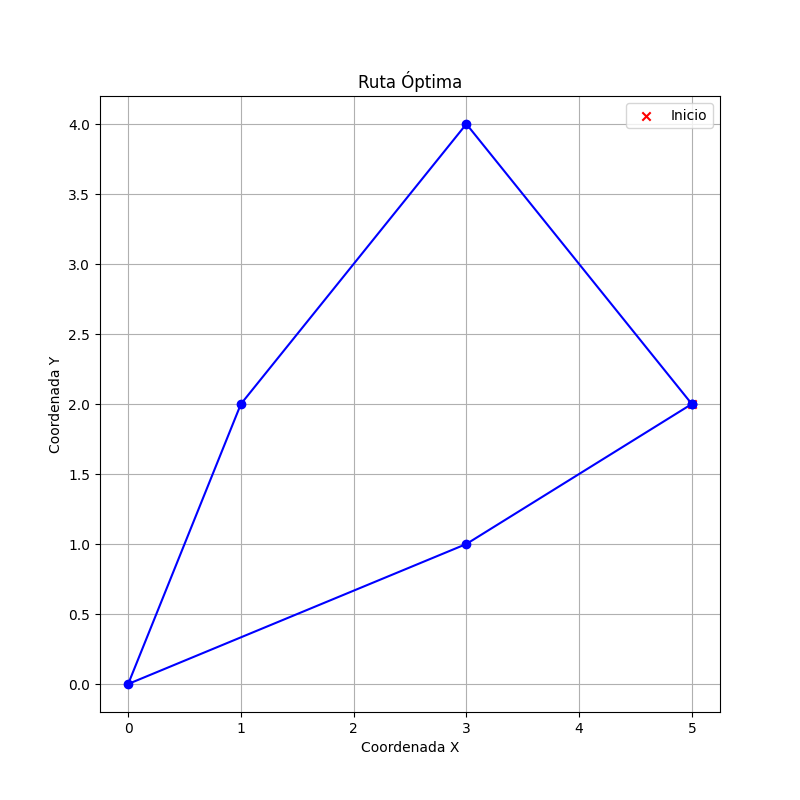
\includegraphics[width=9cm]{img/5Ruta.png}
    \caption{Ruta óptima de la quinta iteración.}
    \label{fig:etiqueta2}
  \end{figure}

\newpage
\subsection{Resultados de procesamiento del Segundo Grupo}

Como observamos en el Cuadro 5, para el segundo grupo se realizaron 10 iteraciones, en donde si encontramos variaciones, ya que el conjunto de datos es de 10 ciudades, haciendo mas compleja la busqueda de una ruta aceptable haciendo el resultado variable.\\

\begin{table}[h]
  \centering
  \caption{Resultados de procesamiento del Segundo Grupo}
  \begin{tabular}{|c|c|c|c|c|}
    \hline
    \textbf{Nro} & \textbf{P. Inicio} & \textbf{Orden de Visita} & \textbf{Distancia} & \textbf{Tiempo (s)}\\
    \hline
    1 & D: [5, 2] & D, G, F, J, I, H, E, B, A, C & 30.1133 & 1.4898 \\
    \hline
    2 & F: [8, 7] & F, G, D, C, A, B, E, H, I, J & 30.1133 & 1.4713 \\
    \hline
    3 & J: [7, 9] & J, I, H, B, A, C, D, E, G, F & 31.6411 & 1.3995 \\
    \hline
    4 & B: [1, 2] & B, A, C, D, E, G, F, J, I, H & 31.6411 & 1.3410 \\
    \hline
    5 & F: [8, 7] & F, J, I, H, E, B, A, C, D, G & 30.1133 & 1.3133 \\
    \hline
    6 & E: [3, 4] & E, B, A, C, D, G, F, J, I, H & 30.1133 & 1.4520 \\
    \hline
    7 & A: [0, 0] & A, C, D, G, F, J, I, H, E, B & 30.1133 & 1.4499 \\
    \hline
    8 & B: [1, 2] & B, E, H, I, J, F, G, D, C, A & 30.1133 & 1.3315 \\
    \hline
    9 & I: [3, 10]& I, H, G, E, B, A, C, D, F, J & 34.4746 & 1.4359 \\
    \hline
    10 & A: [0, 0] & A, C, D, G, F, J, I, H, E, B & 30.1133 & 1.3199 \\
    \hline
  \end{tabular}
\end{table}

En el cuadro anterior observamos como la distancia optima para realizar el recorrido, asi como el tiempo de procesamiento han variado, ya que esta vez las ciudades a recorrer son 10, siento la mejor distancia aceptable 30.1133 y la maxima distancia aceptable 34.4746, con una media de procesamiento de 1.4004 segundos.\\

En cuanto a la evolucion de la mejor distancia podemos observar como esta va cambiando en cada generacion hasta llegar a un punto donde ya no  mejora como podemos ver en la Figura 3.\\
\begin{figure}[h]
\centering
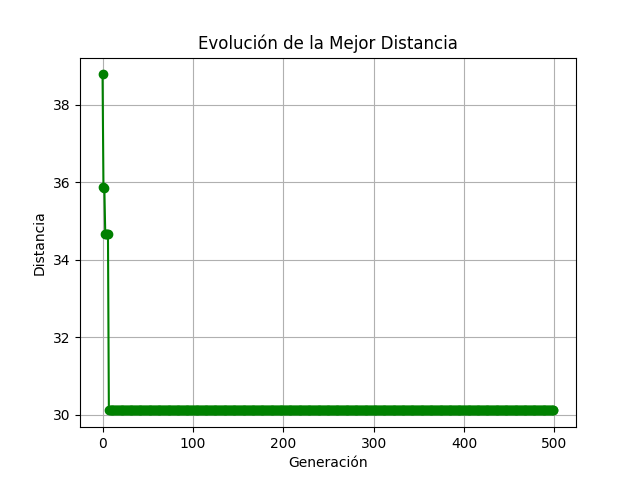
\includegraphics[width=9cm]{img/101Generacion.png}
\caption{Evolución de la mejor distancia en la primera iteración.}
\label{fig:etiqueta3}
\end{figure}
\newpage

\begin{figure}[h]
  \centering
  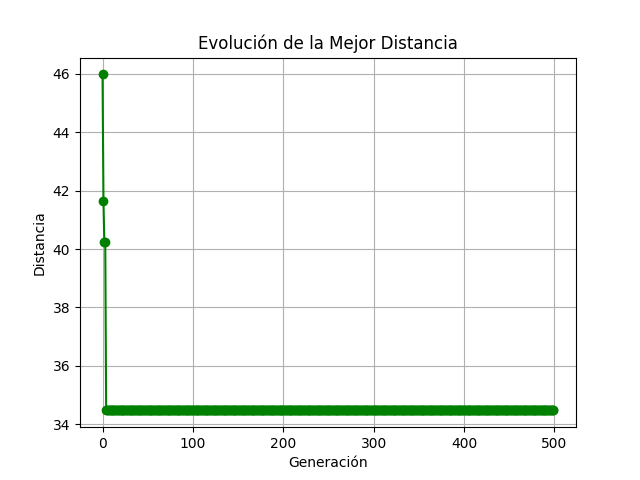
\includegraphics[width=9cm]{img/109Generacion.png}
  \caption{Evolución de la mejor distancia en la novena iteración.}
  \label{fig:etiqueta4}
\end{figure}

Por ultimo en cuanto a la creacion de la ruta óptima podemos apreciar como esta al aumentar el numero de ciudades a visitar sufre variaciones en busqueda de la mejor ruta posible.

\begin{figure}[h]
\centering
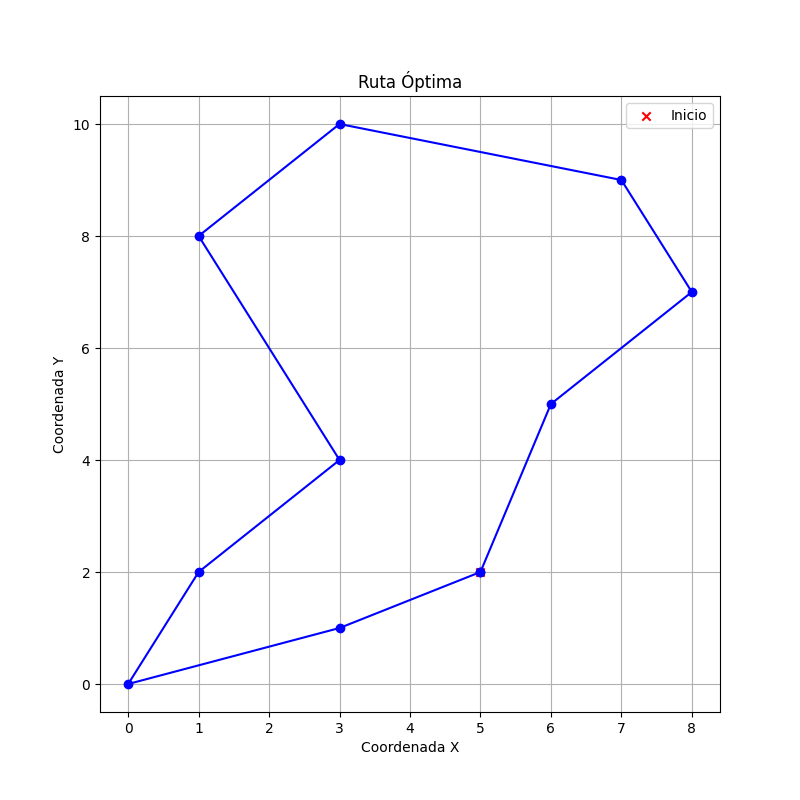
\includegraphics[width=9cm]{img/101Ruta.png}
\caption{Ruta óptima de la primera iteración.}
\label{fig:etiqueta5}
\end{figure}

\begin{figure}[h]
  \centering
  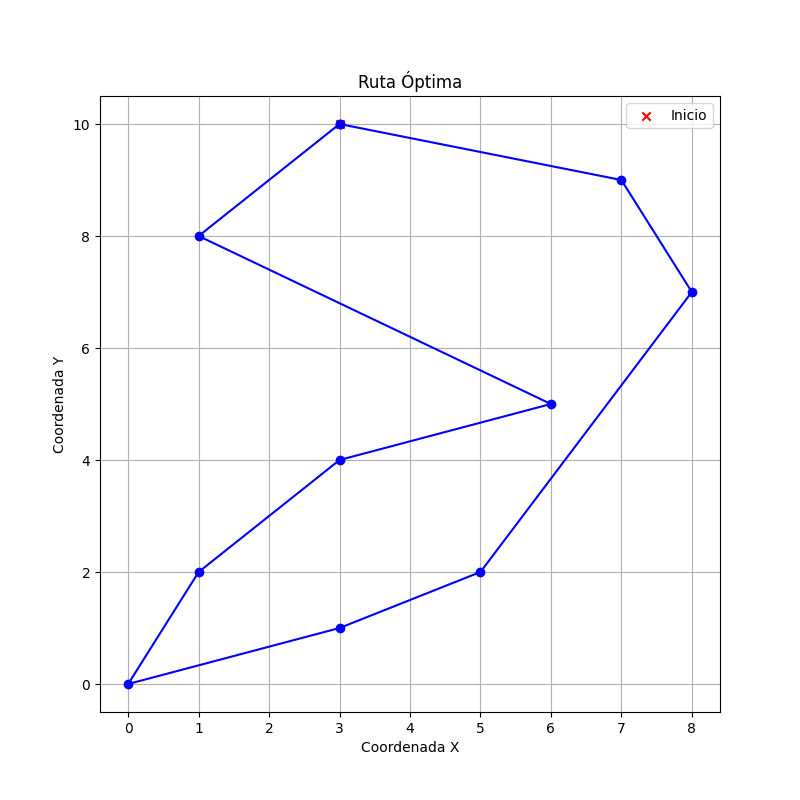
\includegraphics[width=9cm]{img/109Ruta.png}
  \caption{Ruta óptima de la novena iteración.}
  \label{fig:etiqueta6}
\end{figure}

\clearpage
\subsection{Resultados de procesamiento del Tercer Grupo}

Por ultimo, para el tercer grupo de 20 ciudades tambien se realizaron 10 iteraciones en donde la dificultad para encontrar la ruta optima entre las generaciones se elevo, dando los resultados obtenidos en el Cuadro 6.\\

  \begin{table}[h]
    \centering
    \caption{Resultado de procesamiento del Tercer Grupo}
    \begin{tabular}{|c|c | p{6cm} |c|c|}
      \hline
      \textbf{Nro} & \textbf{P. Inicio} & \textbf{Orden de Visita} & \textbf{Distancia} & \textbf{Tiempo (s)}\\
      \hline
      1 & T: [4, 7] & T, D, Q, C, A, K, B, E, R, S, H, N, J, F, P, G, L, O, I, M & 52.3898 & 2.6521 \\
      \hline
      2 & M: [3, 9] & M, S, R, H, O, I, T, L, G, P, Q, D, C, A, K, B, E, F, J, N & 48.6087 & 2.7606 \\
      \hline
      3 & H: [1, 8] & H, M, I, O, N, G, P, Q, D, C, B, R, S, T, J, F, L, E, A, K & 54.8528 & 2.7292 \\
      \hline
      4 & Q: [6, 1] & Q, C, A, K, B, R, S, H, T, L, G, F, J, N, O, I, M, E, D, P & 45.8186 & 2.6659 \\
      \hline
      5 & R: [1, 5] & R, B, K, A, C, G, L, T, M, I, O, N, J, F, P, Q, D, E, S, H & 46.3000 & 2.6411 \\
      \hline
      6 & S: [2, 6] & S, H, O, I, M, T, N, J, F, G, L, E, B, K, A, C, Q, P, D, R & 47.8384 & 2.5960 \\
      \hline
      7 & T: [4, 7] & T, L, G, Q, P, F, J, N, O, I, M, H, S, R, E, D, C, A, K, B & 47.3671 & 2.6121 \\
      \hline
      8 & S: [2, 6] & S, T, L, G, P, Q, D, C, A, K, B, E, F, J, N, O, I, M, H, R & 44.1508 & 2.5910 \\
      \hline
      9 & F: [8, 7] & F, J, N, O, I, M, L, G, P, Q, D, C, A, K, B, E, R, S, H, T & 44.6734 &	2.5761 \\
      \hline
      10 & I: [3, 10] & I, O, N, J, F, L, G, P, Q, D, C, A, K, B, E, R, S, H, T, M & 42.4662 & 2.6297 \\
      \hline
    \end{tabular}
  \end{table}

 Como observamos en el cuadro anterior, la busqueda de la mejor ruta varia notablemente frente a los grupos anteriores, siendo la mejor distancia optima la de 42.4662, mientras que por otro lado tenemos 54.8528 como la distancia mas larga, con una media de procesamiento de 2.6609 segundos.\\

 En cuanto a la evolucion de la mejor distancia en la Figura   podemos apreciar como esta varia al paso de cada generacion en busqueda de una distancia aceptable como solucion al problema.
  \begin{figure}[h]
    \centering
    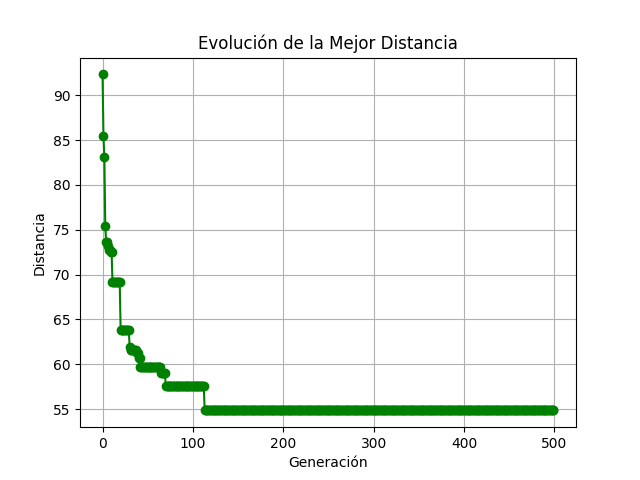
\includegraphics[width=9cm]{img/203Generacion.png}
    \caption{Evolución de la mejor distancia en la tercera iteración.}
    \label{fig:etiqueta7}
  \end{figure}
  
  \begin{figure}[h]
    \centering
    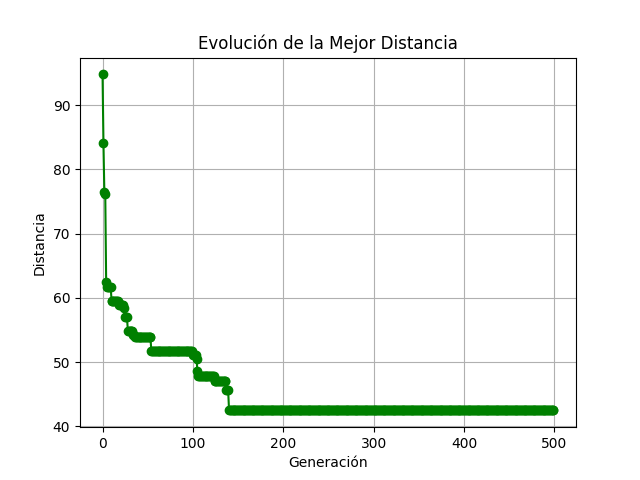
\includegraphics[width=9cm]{img/2015Generacion.png}
    \caption{Evolución de la mejor distancia en la decima iteración.}
    \label{fig:etiqueta8}
  \end{figure}

  \newpage
  Por último, podemos apreciar como las rutas obtenidas a lo largo de las iteraciones varian ampliamente en cada iteración, esto debido al aumento de ciudades a visitar como parte del problema.
  \begin{figure}[h]
    \centering
    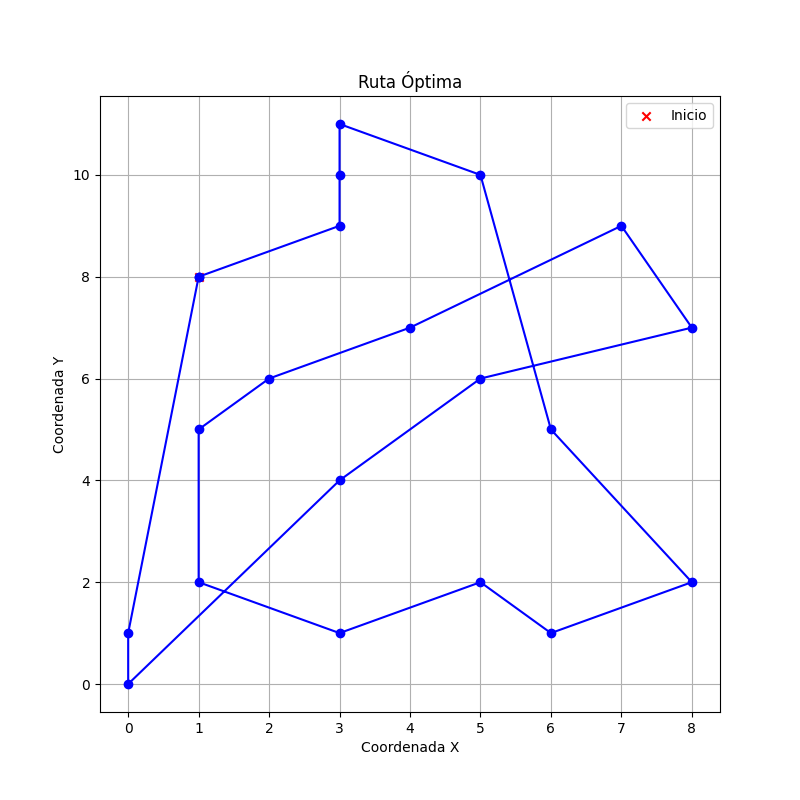
\includegraphics[width=9cm]{img/203Ruta.png}
    \caption{Evolución de la mejor distancia en la tercera iteración.}
    \label{fig:etiqueta9}
  \end{figure}

  
  \begin{figure}[h]
    \centering
    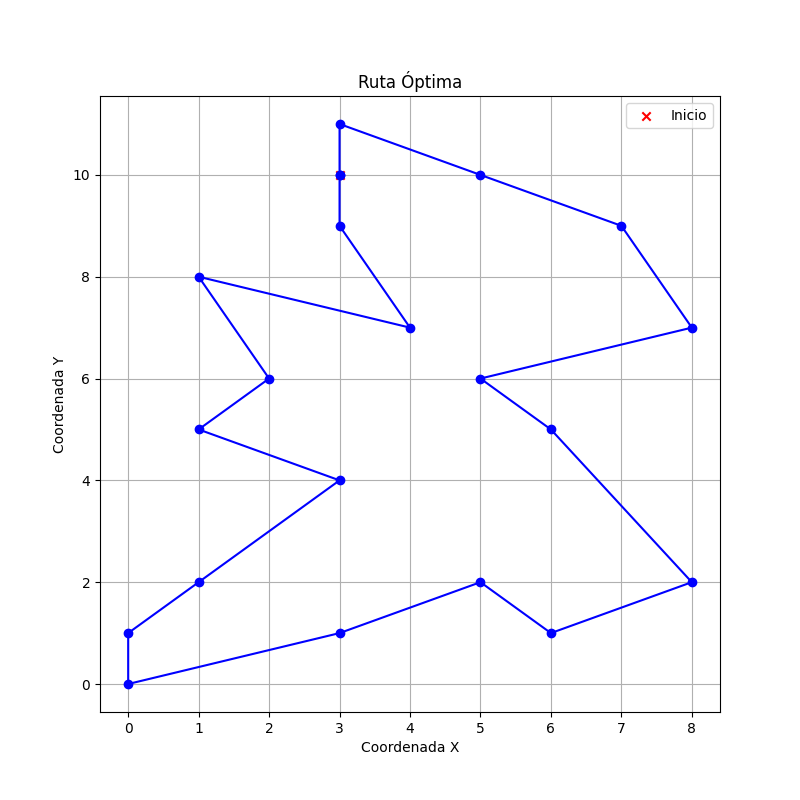
\includegraphics[width=9cm]{img/2015Ruta.png}
    \caption{Evolución de la mejor distancia en la decima iteración.}
    \label{fig:etiqueta10}
  \end{figure}


\clearpage
\section{Conclusiones}

  \begin{itemize}
    \item Como podemos apreciar de los resultados obtenidos en cada  uno de los grupos de prueba es distinto, siendo que los grupos de con mas ciudades los que muestran mayor opciones rutas aceptables como solución al problema.
    \item El aumentar el numero de generacion al procesamiento del algoritmo no garantiza encontrar la mejor solución.
    \item La aplicación de un algoritmo genético lorga brindar una solucion al problema con un costo computacional aceptable, a diferencia de un algoritmo exacto.
  \end{itemize}
\end{document}
